\documentclass[journal,comsoc]{IEEEtran}
\usepackage{algorithm}
\usepackage{algpseudocode}
\usepackage{graphicx}
\usepackage{float}
\usepackage{multirow}
\usepackage{tabularx}
\usepackage{caption}
\usepackage{array}
\usepackage{enumitem}

\setlength{\parskip}{1em}
\begin{document}

\title{\Large
Predictive Modeling and Explainable AI Analysis of Farm Features and Practices 
Impacting White Spot Disease Prevalence in Farmed Shrimps in Bangladesh}
\author{
Authors:
Al Ibne Siam, 
Rafeed Mohammad Sultan, 
Istiaque Hasan Nihal, 
Mohammed Arif Uddin 
}
\maketitle

\begin{abstract}
White Spot Disease (WSD) is a highly contagious viral infection that can lead to the rapid death of crustacean (shrimp, crab, prawn, etc.) populations. In our study, we implemented different machine-learning tools and algorithms to predict whether the prevalence of WSD in farmed shrimp will increase, decrease, or remain unchanged based on the features of shrimp farms in Bangladesh and their associated farming practices. We achieved an accuracy of 72.08\%.

Furthermore, we used SHAP (SHapley Additive exPlanations) explainable AI to discover the effects of different farm features and practices on the change in prevalence, offering valuable insights into various trends in the data. Hence, this research has the potential to help minimize the prevalence of White Spot Disease in farmed shrimps in Bangladesh.
\end{abstract}


\begin{IEEEkeywords}
Keywords: White Spot Disease, White Spot Syndrome Virus, Shrimp Farming, Shrimp Farming Bangladesh
\end{IEEEkeywords}

\section{Introduction}
White Spot Disease (WSD) (Fig. 1), caused by the White Spot Syndrome Virus (WSSV), is a major threat to crustacean lives. It is highly contagious and, if left untreated, can lead to rapid deaths in crustacean populations. Contaminated water or infected crustaceans are the primary sources of this disease.  

WSD is widespread in farmed shrimps of Bangladesh. A study conducted in 2015 $^{[1]}$ reported that the prevalence of the disease in farmed shrimp was 79\% in Satkhira, 50\% in Khulna, 38\% in Bagerhat, and 25\% in Cox's Bazar. Limiting the prevalence of White Spot Disease is crucial and, nevertheless, a big challenge for the aquaculture industry of Bangladesh.

\begin{figure}[H]
  \centering
  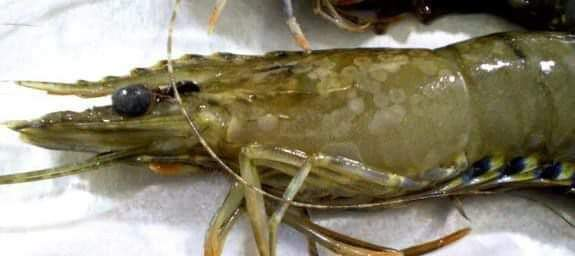
\includegraphics[width=0.4\textwidth]{shrimp.jpg}
  \caption{White Spot Disease in Shrimp}
  \label{fig:shrimp}
\end{figure}

The objective of our study is to explore the feasibility of employing machine learning tools and algorithms to mitigate this disease. Our approach involves predicting the influence of farm features and practices on the incidence of White Spot Disease (WSD), followed by applying explainable AI to analyze the impact of various factors on its prevalence. For our problem, we used the “Dataset of white spot disease affected shrimp farmers disaggregated by the variables of farm site, environment, disease history, operational practices, and saline zones” dataset $^{[2]}$ from the Department of Aquaculture, Bangladesh Agricultural University, Mymensingh, Bangladesh. It consists of many farming features and practices which were deemed to be relevant to shrimp farming. The data was collected from 233 farms affected by WSSV across the Khulna, Bagerhat, and Satkhira districts of Bangladesh.

At first, we employed three machine learning algorithms: a Random Forest Classifier, a K-Nearest Neighbor classifier, and a Naive Bayes classifier to forecast whether the disease's prevalence will increase, decrease, or remain stable. After an initial filter feature selection, we repeatedly conducted feature selection for each ML classifier based on importance and fine-tuned the hyperparameters to get the highest accuracy. Then, we created an ensemble model that combines the Random Forest (RF), K-Nearest Neighbor (KNN), and Naive Bayes (NB) classifiers. Given the limited size of our dataset, we assessed accuracy using a 10-fold stratified cross-validation test and computed the mean accuracy as the performance metric. We then performed a comparative analysis of the different models. Finally, we selected the model with the highest accuracy and applied SHAP explainable AI to analyze trends in relation to the selected features for that model.

In the subsequent sections of our report, we will discuss relevant studies in the existing literature, introduce the dataset, explain the methodology, present our results, and conduct a detailed research analysis.


\section{Related Work}
Most studies in the literature related to White Spot Disease in shrimps are medical studies analyzing the disease. Nevertheless, there are a few relevant studies using machine learning.

A study on the same dataset by Edeh et al. $^{[3]}$ mistakenly identified WSD presence to be in farmers rather than in the shrimp population, as mentioned in the document accompanying the dataset. It predicted the presence or absence of the disease, using Bootstrapping of Random Forest and CHAID (Chi-squared Automatic Interaction Detection), and achieved an accuracy of 98.28\%.

Another study $^{[4]}$ used the continuous diphasic model (CDM) to predict survival percentage over time following white spot disease (WSD) outbreaks in shrimp populations, offering enhanced modeling capabilities compared to the discontinuous diphasic model (DDM).

A final type of study is using image classification to segregate healthy shrimps from infected ones. One such study, “A Novel Neural Network Model for Shrimp Segmentation to Detect White Spot Syndrome,” $^{[5]}$ uses Canny–GLCM (Gray Level Co-occurrence Matrix) incorporated with a simple Artificial Neural Network (ANN) and achieved accuracy of 94.67\%, sensitivity of 94.79\% and specificity of 94.51\%.

Our dataset is new and novel, so research is scarce in this area where farming practices were considered for White Spot Disease prediction in shrimps. The study by Edeh et al. $^{[3]}$ only predicted the presence of the disease, which is a much simpler task. Predicting the type of change in the prevalence of WSD is more important. Hence, our work emerges as a novel contribution to the field.

\section{Methodology}
\subsection{Exploring the dataset}
Our dataset $^{[2]}$ is an Excel file comprising 46 variables and 233 data samples collected from 233 shrimp farms of different sizes from Khulna, Bagerhat, and Satkhira. It contains three types of data: continuous, nominal, and binary, across these categories: socio-economic factors, farm characteristics, environmental attributes, and disease history. Our study primarily focuses on farm characteristics, environmental attributes, and disease history.
 

\subsection{Generating label}
Disease history consists of the prevalence of WSD in the culture of the previous session and the prevalence of WSD in the culture of the current session. Using these values, we will generate our target: the type of change in the prevalence of WSD in the shrimp population.

We classify changes in prevalence into three distinct classes:
\begin{itemize}
  \item Class -1: There was a decrease of at least 10\%
  \item Class 0: Change in prevalence was less than 10\%
  \item Class 1: There was an increase of at least 10\%
\end{itemize}
We generated a new column for our label called “change.” Algorithm 1 demonstrates our implementation of label generation.

\begin{algorithm}[H]
\caption{Label generation}
\begin{algorithmic}
\State
\State $current\_prev \gets$ the current prevalence
\State $previous\_prev \gets$ the previous prevalence
\State $change \gets 0$
\If{$current\_prev \leq 0.9 \cdot previous\_prev$}
    \State $change \gets -1$
\ElsIf{$current\_prev \geq 1.1 \cdot previous\_prev$}
    \State $change \gets 1$
\Else
    \State $change \gets 0$
\EndIf
\State
\end{algorithmic}
\end{algorithm}

\subsection{Handling missing values}
Analyzing the dataset, we find that the only columns missing values are “Temperature”, “pH”, and “Salinity.” 

Since they are all continuous variables from environment variables, we could use the mean of all the values in the columns. However, the mean across all values is likely less accurate than that across all the values for the corresponding zone in which the farm with the missing value belongs.

Hence, instead of a “global mean,” we used a “zonal mean” to fill the missing values. Algorithm 2 demonstrates our process of handling null values for continuous features with missing values.

\begin{algorithm}
\caption{Fill Nulls with Zonal Mean}
\begin{algorithmic}
\State
\Function{FillNullsWithZonalMean}{$df$, $col$}
    \State $grouped\_zones \gets df.\text{groupby}('Zone')$
    \State $zonal\_mean \gets$ \\
    \hspace{5em}$grouped\_zones[col].\text{transform}('mean')$
    \State $df[col].\text{fillna}(zonal\_mean, \text{inplace}=\text{True})$
    \State \Return $df$
\EndFunction
\State
\end{algorithmic}
\end{algorithm}

\subsection{Dimensionality reduction via statistical filter based feature selection}
At first we conducted an initial round of dimensionality reduction to eliminate the features with poor correlation or impact on our target variables. 

For continuous features, We calculated eta-squared values to identify the influence of continuous variables on the label, characterized by eta-squared values ranging from medium effect (\textgreater 0.06) to large effect (\textgreater 0.14). Following that, we dropped features with very poor eta-squared coefficients (\textless 0.01), which resulted in the elimination of the “PeriodOfFallow.”

For our categorical features (binary and nominal features), we calculated the Cramer’s V coefficient as a measure of association between the features and target variables. Following that, we dropped features with very poor correlation coefficients (\textless 0.1), which resulted in the elimination of  'GherDryAfterHarvest,' 'WaterComingViaOtherFarms,' 'CropRotation,' 'ChemicalUsePondPreparation,' 'SludgeRemovalInterval,' 'MaintainAndRepairDikes,' 'WaterSource\_IndirectNatural.'

\subsection{Preprocessing the data}
\subsubsection{One-Hot Encoding of Nominal Features}
Nominal attributes were transformed using one-hot encoding. This technique allows for representing categorical variables as binary vectors, enabling models to interpret better and utilize this information. For each nominal attribute identified, a set of binary columns was created, with each column corresponding to a unique category within the attribute. 

We defined the function one\_hot\_encode\_and\_rename for this purpose. It iterates through the specified nominal columns, applies one-hot encoding using the pd.get\_dummies() function, and appends the resulting binary columns to the dataset. The original nominal column is subsequently removed. The name of the generated columns followed the format: \textless feature\_name \textgreater\_\textless value \textgreater

\subsubsection{Normalization of Continuous Features}

Continuous variables were scaled to a standard range to mitigate disparities in magnitude, which can affect the performance of machine learning algorithms. The Min-Max scaling technique transformed continuous variables to the interval [0, 1]. This ensures that all features contribute proportionally to the learning process.
We defined the function normalize\_continuous\_variables for this task. It iterates through the continuous columns and applies Min-Max scaling. The scaled values are then updated in the data frame.

\subsection{Building models, Importance-based feature selection, and Hyperparameter Optimization}
\subsubsection{Random Forest Classifier}

In this section, we employ the Random Forest Classifier to construct predictive models for our dataset. The methodology involves several key steps to ensure robust model performance.

Importance-based Feature Score Generation:

To gain insights into the contribution of each feature towards the predictive power of the model, we computed feature importance scores using a Random Forest Classifier trained on the entire preprocessed dataset.

Optimal Parameter Search:

To determine the most effective combination of features and hyperparameters, we conducted an exhaustive search across a range of threshold values for feature selection and varying numbers of estimators. The goal was to identify the threshold value and number of estimators that yielded the highest mean accuracy across 10-fold cross-validation. The results of this search were visualized in a heatmap, providing a comprehensive view of the parameter space and its impact on model performance.

Final Model Tuning:

Through iterative hyperparameter fine-tuning and feature selection, we repeatedly conducted a grid search, taking a range of values of thresholds and the number of estimators. After each search, we continued the grid search by exploring the unexplored values in the range where our optimum threshold and hyperparameter values reside. The process was repeated until we arrived at a single set of optimal values for the threshold and number of estimators. The heat maps of the grid searches are provided in Fig. 2 - 4.

\begin{figure}[H]
  \centering
  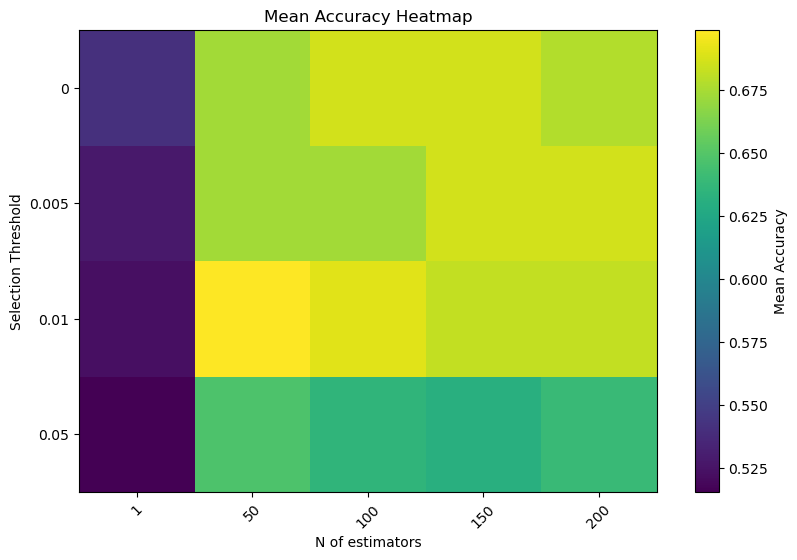
\includegraphics[width=0.4\textwidth]{rf_grid_search_1.png}
  \caption{First grid search for Random Forest Classifier}
  \label{fig:rf_grid_search_1}
\end{figure}

\begin{figure}[H]
  \centering
  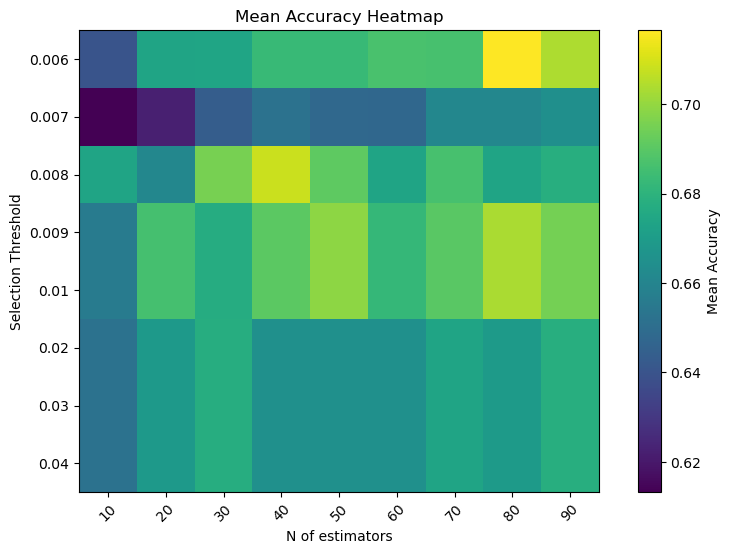
\includegraphics[width=0.4\textwidth]{rf_grid_search_2.png}
  \caption{Second grid search for Random Forest Classifier}
  \label{fig:rf_grid_search_2}
\end{figure}

\begin{figure}[H]
  \centering
  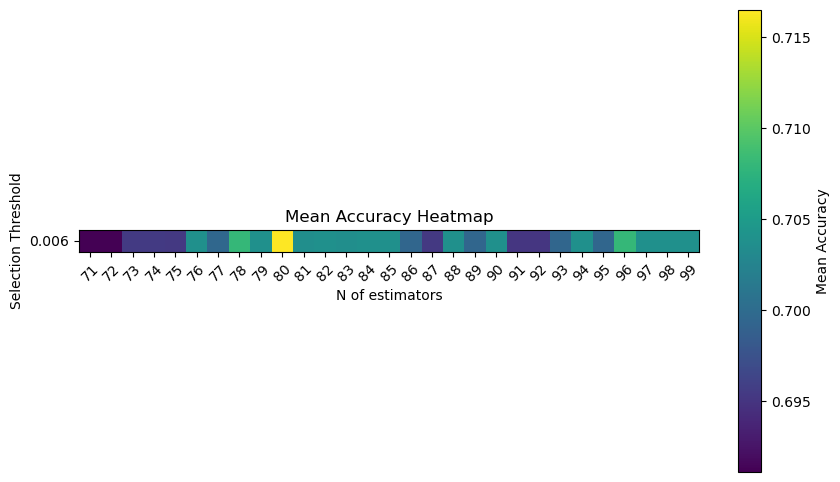
\includegraphics[width=0.4\textwidth]{rf_grid_search_3.png}
  \caption{Final grid search for Random Forest Classifier}
  \label{fig:rf_grid_search_3}
\end{figure}

From these grid searches, we find that the Random forest classifier performs best when working with the top 44 (threshold \textgreater 0.06) features instead of the 56 features we obtained after dataset preprocessing. The optimum number of estimators is 80 for this model.

The combination of importance-based feature selection and hyperparameter optimization ensures that the Random Forest Classifier is tailored to the specific characteristics of our dataset, resulting in a robust and accurate predictive model.

\subsubsection{KNN Classifier}
In this section, we detail the process of constructing K-Nearest Neighbors (KNN) classifiers, focusing on feature selection and optimal number of neighbors selection for both uniform and distance-based voting.

Feature Selection with SelectKBest:

The SelectKBest algorithm was employed to identify the most informative features using the analysis of variance test (ANOVA). By varying the parameter 'k,' we obtained sets of top 'k' features with the most importance.

Optimal Number of Neighbors:

For each set of selected features, an exhaustive search was conducted to identify the optimal number of neighbors ('k') for the KNN classifier. Through cross-validation, we assessed the classifier's performance with varying numbers of neighbors and recorded the mean accuracy scores.

We performed the entire process twice, once for uniform voting and once for distance-based voting, to account for different voting strategies in the KNN algorithm. This comparative analysis allowed us to select the optimal configuration for our specific dataset.

Similar to the Random Forest Classifier, we conducted a grid search, taking a range of values of “k” for the top k features selection and the number of neighbors. After each search, we continued the grid search by exploring the unexplored values in the range where our optimum k and hyperparameter values reside. Our find is illustrated Fig. 5-8.

\begin{figure}[H]
  \centering
  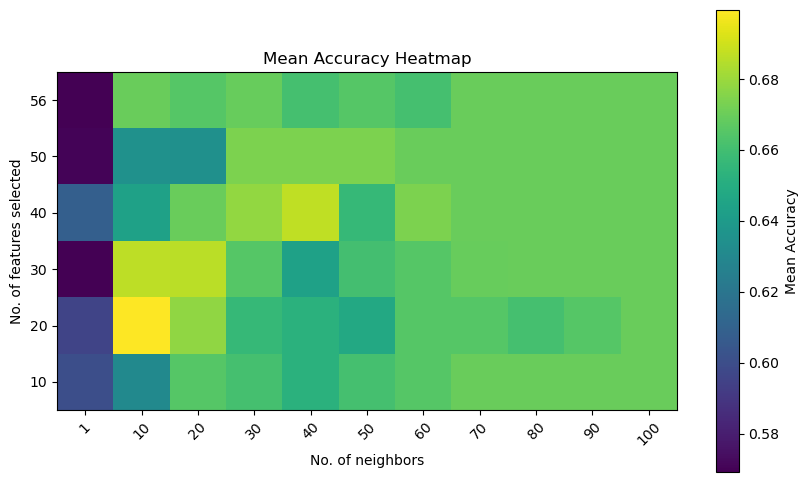
\includegraphics[width=0.4\textwidth]{knn1.png}
  \captionsetup{font=small} % Adjust the font size here (small, footnotesize, etc.)
  \caption{First grid search for KNN classifier with uniform voting}
  \label{fig:knn1}
\end{figure}
\vspace{-20pt} 

\begin{figure}[H]
  \centering
  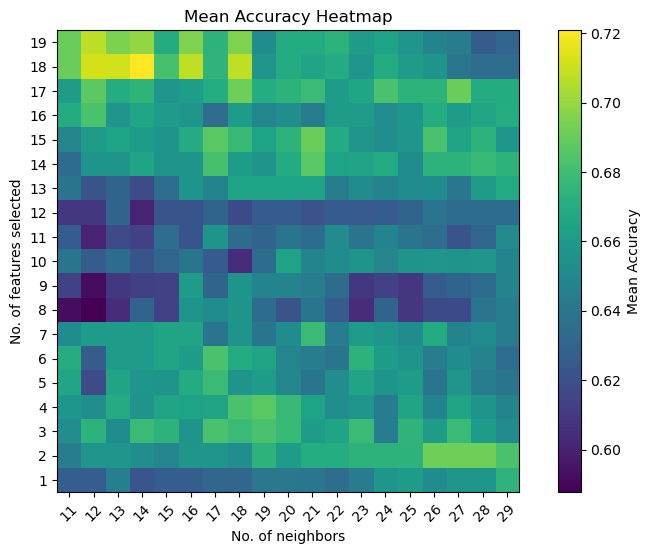
\includegraphics[width=0.4\textwidth]{knn3.png}
  \captionsetup{font=small} % Adjust the font size here (small, footnotesize, etc.)
  \caption{Final grid search for KNN classifier with uniform voting}
  \label{fig:knn3}
\end{figure}


\begin{figure}[H]
  \centering
  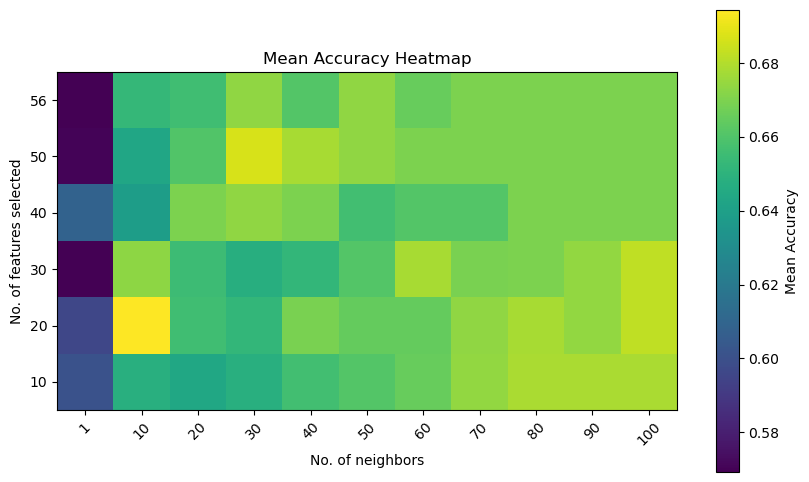
\includegraphics[width=0.4\textwidth]{knn2.png}
  \captionsetup{font=small} % Adjust the font size here (small, footnotesize, etc.)
  \caption{First grid search for KNN classifier with distance-based voting}
  \label{fig:knn2}
\end{figure}
\vspace{-20pt} 

\begin{figure}[H]
  \centering
  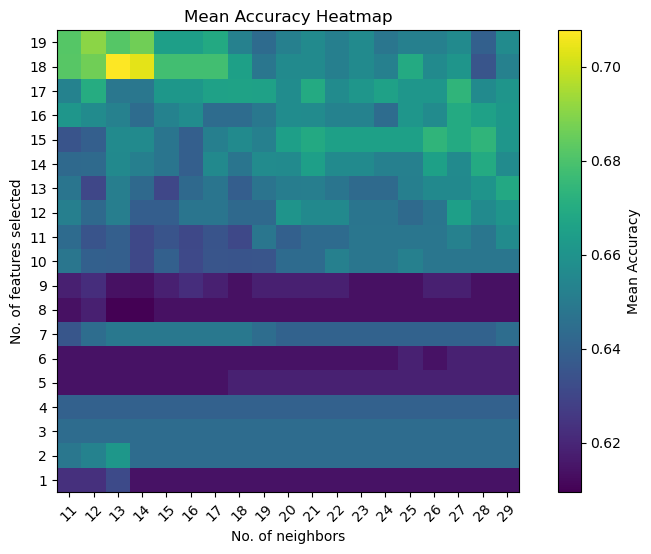
\includegraphics[width=0.4\textwidth]{knn4.png}
  \captionsetup{font=small} % Adjust the font size here (small, footnotesize, etc.)
  \caption{Final grid search for KNN classifier with distance-based voting}
  \label{fig:knn4}
\end{figure}

For the KNNr classifier, our model performed best when trained on the top 18 best features and doing uniform votes from the nearest 14 neighbors.

\subsubsection{Multinomial Naive Bayes Classifier}
In this section, we describe the methodology employed to construct the Multinomial Naive Bayes classifier.

Feature Selection and Hyperparameter Optimization:

We employed the SelectKBest algorithm to identify the most relevant features for the Multinomial Naive Bayes classifier. Varying values of 'k' allowed us to obtain subsets of features.

Fine-Tuning Hyperparameters:

We conducted a fine-tuning process around the optimal values to further enhance the performance of the Multinomial Naive Bayes classifier. We repeatedly conducted grid searches to find the best set of features and alpha. Similar to the classifier before, after each search, we explored the unexplored values around our optimum k and alpha values. The heat maps of the grid searches are shown in Fig. 9-10.

\begin{figure}[H]
  \centering
  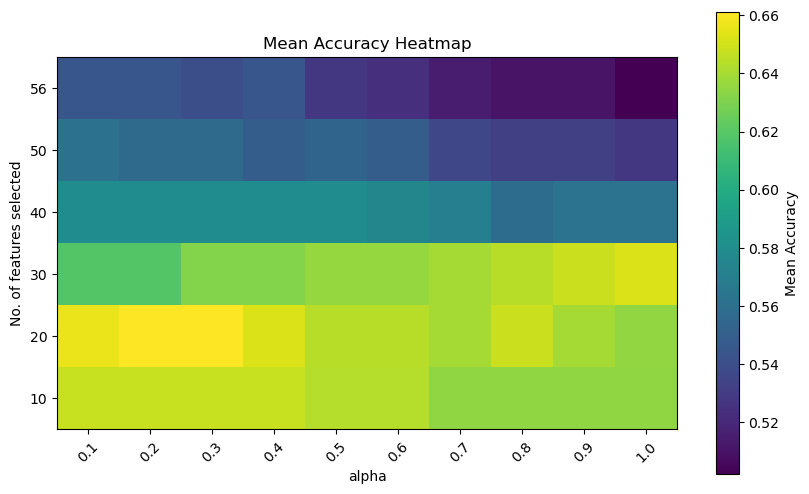
\includegraphics[width=0.4\textwidth]{nb1.png}
  \caption{ First grid search for Multinomial Naive Bayes classifier.}
  \label{fig:nb1}
\end{figure}

\begin{figure}[H]
  \centering
  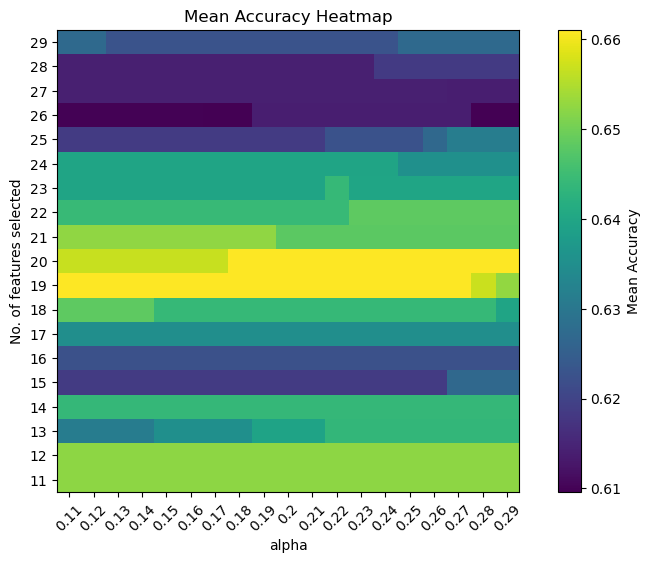
\includegraphics[width=0.4\textwidth]{nb2.png}
  \caption{Final grid search for Multinomial Naive Bayes classifier.}
  \label{fig:nb2}
\end{figure}

From these grid searches, we obtained the best Multinomial Naive Bayes Classifier using the top 19 best features, using an alpha value of 0.11. Since the alpha value can go to an indefinite level of precision, we decided to limit our investigation to two grid searches.

\subsubsection{An Ensemble of All our Classifiers}
We ensembled three classifiers (Random Forest, K-Nearest Neighbors, and Multinomial Naive Bayes) using their respective optimal hyperparameters and selected features. The ensemble method combined the classifiers' predictions, with K-Nearest Neighbors taking precedence in cases of ties. The final mean accuracy across a 10-fold stratified cross-validation test was calculated. Algorithm 3 demonstrates our voting process.


\begin{algorithm}
\caption{Ensemble Voting Algorithm}
\begin{algorithmic}
\State
\State $preds \gets [rf\_pred, knn\_pred, nb\_pred]$
\State $set\_of\_pred \gets \text{set}(preds)$

\If{$\text{length of } set\_of\_pred == 3$}
    \State $final\_pred \gets preds[1]$
\Else
    \State $final\_pred \gets \text{max}(set\_of\_pred, \text{key} = \text{preds.count})$
\EndIf
\State
\end{algorithmic}
\end{algorithm}

\section{Test Results}
\subsection{Performance of different models}
Taking into account the small sample size of our dataset, we decided to conduct 10-fold stratified cross-validation tests instead of the traditional train test split for our research. This will give us a more robust and comprehensive depiction of our models' performances.

Three different classifiers—Random Forest, K-Nearest Neighbors (KNN), and Multinomial Naive Bayes—as well as an ensemble of these classifiers, were applied in our research. The results are listed in the Table 1.

\begin{table}[H]
    \centering
  \captionsetup{labelsep=none}
  \renewcommand{\arraystretch}{1.5}
  \begin{tabularx}{8.75cm}{|>{\centering\arraybackslash}p{1.5cm}|>{\centering\arraybackslash}p{1cm}|>{\centering\arraybackslash}p{2.25cm}|>{\centering\arraybackslash}p{2.25cm}|}
    \hline
    \textbf{Model} & \textbf{Accuracy} & \textbf{Optimal Hyperparameters} & \textbf{Optimal Feature Selection} \\
    \hline
    Random Forest & 71.65\% & 80 estimators & Importance score \textgreater 0.06 (44 features selected) \\
    \hline
    K-Nearest Neighbor & 72.08\% & 1. Uniform voting\newline 2. Voting with 14 nearest neighbors & 18 best features selected \\
    \hline
    Multinomial Naive-Bayes & 66.11\% & $\alpha = 0.11$ & 19 best features selected \\
    \hline
    Ensemble of the three & 71.67\% & For each classifier, their respective optimal hyperparameters were used & For each classifier, their respective optimal set of features was used \\
    \hline
  \end{tabularx}
  \caption{ : Model Performances}
  \label{tab:model-performance}
\end{table}


\subsection{Explainable AI result}
The XAI analysis was done on the KNN Model as it performed the best as an individual classifier, incorporating it's optimal hyperparameters and optimal set of 18 features.

We used SHAP XAI library for this purpose. SHAP is a powerful tool that provides a detailed account of feature importance and how each feature impacts the model’s predictions. 

 We divided our data using a 75-25 target stratified split, where 75\% of the samples were used as background and training data and 25\% of the samples were used for predictions when generating SHAP values. We employed SHAP by creating a Kernal Explainer, which produces Shapley values plotted in the figure below. 

\begin{figure}[H]
  \centering
  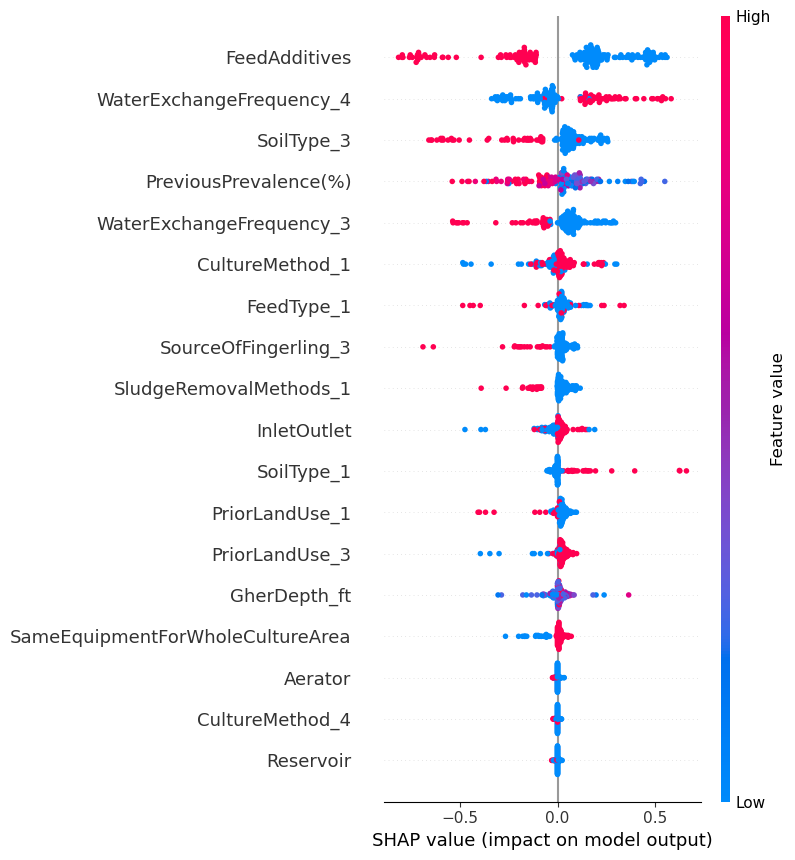
\includegraphics[width=0.4\textwidth]{XAI.png}
  \caption{Shapley values for different features}
  \label{fig:xai}
\end{figure}

\section{ Discussion and Analysis}
\subsection{Analysis of the performance}
From individual classifiers, KNN performed the best, outperforming Random Forest by a small margin, while using much fewer features (18 as opposed to 44 by RF). Naive Bayes performed the worst and by a considerable margin. The ensemble of the three models performed better than the Random Forest classifier but could not improve on the performance of the KNN classifier.

\subsection{Analysis of XAI}
The graphical plot denoted some trends:

\begin{enumerate}[itemsep=10pt]
    \item Feed additives: The use of feed additives tends to have a significant impact in lowering the prevalence of WSD.
    
    \item Water exchange: Water exchange frequency of \textless7 - 28 days (water exchange 4) tends to have a significant impact in increasing the prevalence of WSD. Water exchange frequency of every 29-42 days (water exchange 3) tends to have a significant impact in decreasing the prevalence of WSD.
    
    \item Soil type: Clay soil (soil type 1) tends to have a significant impact in increasing the prevalence of WSD. Sandy soil (soil type 3) tends to have a significant impact in decreasing the prevalence of WSD.
    
    \item Culture method: Using a polyculture of shrimp with fish (culture method 1) tends to have a modest impact in increasing the prevalence of WSD. However, the trend is not consistent.
    
    \item Source of fingerling: Using fingerling from the regular hatchery (source of fingerling 3) tends to have a modest impact in decreasing the prevalence of WSD.
    
    \item Sludge Removal Method: Flushing and depositing sludge off the farm (sludge removal method 1) tends to have a modest impact in decreasing the prevalence of WSD.
    
    \item Inlet/Outlet: Using separate passes for water inlet and outlet tends to have a modest impact in decreasing the prevalence of WSD. However, the trend is not consistent.
    
    \item Prior Land Use: If the land was a wetland or other land not used for farming (prior land use 1), it tends to have a modest impact in decreasing the prevalence of WSD. If the land was rich and was used for farming (prior land use 3), it tends to have a modest impact in increasing the prevalence of WSD.
\end{enumerate}

\section{Limitations}
\begin{itemize}[itemsep=10pt]
    \item The dataset we worked with has a very small sample size. Similar datasets could not be found in the literature. Furthermore, it only sampled data from 3 different regions of Bangladesh. Other regions like Coxs Bazar were not considered.

    \item While all our models performed much better than the baseline performance (33\% accuracy), it is still not outstanding. The maximum mean accuracy achieved over 10-fold cross-validation was 72.08%.

    \item One of the trends (number 2), as suggested in the analysis of XAI results, suggests that exchanging water frequently contributes to a higher prevalence of WSD. This sounds counterintuitive, as frequently changing water should decrease disease transmission. This trend could be only specific to this dataset, or it could be possible that the main source of WSSV is the water farmers are using during water exchange. This needs to be further investigated.
\end{itemize}

\section{Conclusions}
In our study, we built different machine-learning models to predict changes in the prevalence of WSD. We achieved a mean accuracy of 72.08\% for the KNN classifier using the top 18 features to make predictions using uniform votes from the 14 nearest neighbors. Random forest classifier with 80 estimators and using the top 44 most important features achieved a mean accuracy of 71.65\%. Multinomial Naive-Bayes using the best 19 features and an alpha value of 0.11 performed the worst, achieving a mean accuracy of 66.11\%. The ensemble of these three models could not improve on the performance of the individual best model, achieving an accuracy of 71.67\%.

From our explainable AI result analysis on our KNN model (best performer), we found different prevalence trends for each feature, which we have discussed above.

Considering the small sample size and less-than-spectacular performance of our model, the findings in our research are important but by no means conclusive. We need more datasets similar to the ones we used, and future research is needed to draw definitive conclusions.

\section*{References}

[1] Anwar Hossain, Shuvro Nandi, Mohammad Siddique, Santonu Sanyal, Munawar Sultana, and Mohammed Hossain, "Prevalence and Distribution of White Spot Syndrome Virus in Cultured Shrimp," Letters in Applied Microbiology, 2015, doi: 10.1111/lam.12353.

[2] Neaz Al Hasan and Mohammad Mahfujul Haque, "Data for: Dataset of white spot disease affected shrimp farmers disaggregated by the variables of farm site, environment, disease history, operational practices, and saline zones," Mendeley Data, 2020, doi: 10.17632/nz96v5spbf.2.

[3] M.O. Edeh, S. Dalal, I.C. Obagbuwa, et al., "Bootstrapping random forest and CHAID for prediction of white spot disease among shrimp farmers," Sci Rep, 2022, doi: 10.1038/s41598-022-25109-1.

[4] Miguel A González‐Romero, Javier M J Ruiz‐Velazco, Margarita Estrada‐Pérez, José T Nieto‐Navarro, Iram Zavala‐Leal, and Alfredo Hernandez‐Llamas, "Assessing uncertainty of semi‐intensive production of whiteleg shrimp (Litopenaeus vannamei) using partial harvesting programs," Aquaculture Research, 2017, doi: 10.1111/are.13542.

[5] Lakshmanan Ramachandran and Veerasamy Mohan, "A Novel Neural Network Model for Shrimp Segmentation to Detect White Spot Syndrome," 2022, pp. 1453–1466.

\end{document}
